\documentclass[journal]{IEEEtran}
\usepackage{amssymb}
\usepackage{amsmath}
\usepackage[colorlinks=true, linkcolor=black]{hyperref} % Links
\usepackage{makeidx} % Indexierung
\usepackage{siunitx}
%\usepackage[ngerman]{babel} % deutsche Sonderzeichen
\usepackage[utf8]{inputenc}
\usepackage{geometry} % Dokumentendesign wie Seiten- oder Zeilenabstand bestimmen
\usepackage{algorithm}
\usepackage{algorithmic}
\usepackage{caption}
\usepackage{subcaption}
%\usepackage[toc,page]{appendix}

% Graphiken
\usepackage{tikz}
\usepackage{pgfplots}
\usepackage{pgfmath}
\usepackage{pgfcore}
\usepackage{pgfopts}
\usepackage{pgfkeys}
\usepackage{pgfornament}
\usepackage{pgf}
\usepackage{ifthen}
\usepackage{booktabs}

% Tabellen
\usepackage{tabu}
\usepackage{longtable}
\usepackage{colortbl} % Tabellen faerben
\usepackage{multirow}
\usepackage{diagbox} % Tabellenzelle diagonal splitten

\usepackage{xcolor} % Farben
\usepackage[framemethod=tikz]{mdframed} % Hintergrunderstellung
\usepackage{enumitem} % Enumerate mit Buchstaben nummerierbar machen
\usepackage{pdfpages}
\usepackage{listings} % Source-Code darstellen
\usepackage{eurosym} % Eurosymbol
\usepackage[square,numbers]{natbib}
\usepackage{here} % figure an richtiger Stelle positionieren
\usepackage{verbatim} % Blockkommentare mit \begin{comment}...\end{comment}
\usepackage{ulem} % \sout{} (durchgestrichener Text)
\usepackage{abstract}
\usepackage{blindtext}
\usepackage{fancyref}

% BibLaTex
\bibliographystyle{acm}

% Aendern des Anhangnamens (Seite und Inhaltsverzeichnis)
%\renewcommand\appendixtocname{Anhang}
%\renewcommand\appendixpagename{Anhang}

% mdframed Style {{{
\mdfdefinestyle{codebox}{
	linewidth=2.5pt,
	linecolor=codebordercolor,
	backgroundcolor=codecolor,
	shadow=true,
	shadowcolor=black!40!white,
	fontcolor=black,
	everyline=true,
}
% }}}

% Seitenabstaende
%\geometry{left=15mm,right=15mm,top=15mm,bottom=20mm}

% TikZ Bibliotheken {{{
\usetikzlibrary{
    arrows,
    arrows.meta,
    decorations,
    backgrounds,
    external,
    positioning,
    fit,
    petri,
    shadows,
    datavisualization.formats.functions,
    calc,
    shapes,
    shapes.multipart,
    matrix
}
% }}}

\pgfplotsset{width=7cm,compat=1.15}

\definecolor{codecolor}{HTML}{EEEEEE}
\definecolor{codebordercolor}{HTML}{CCCCCC}

% Standardeinstellungen fuer Source-Code listings {{{
\lstset{
    language=C,
    breaklines=true,
    keepspaces=true,
    keywordstyle=\bfseries\color{green!70!black},
    basicstyle=\ttfamily\color{black},
    commentstyle=\itshape\color{purple},
    identifierstyle=\color{blue},
    stringstyle=\color{orange},
    showstringspaces=false,
    rulecolor=\color{black},
    tabsize=2,
    escapeinside={\%*}{*\%},
}
% }}}

%\input{libuml}
%\input{liberm}

\title{Partial Classification Forest}

\author{Jonas Fa{\ss}bender \\ [1ex]
  \href{mailto: jonas@fc-web.de}{jonas@fc-web.de}}
\date{}

\begin{document}

\maketitle

\begin{abstract}
  %\noindent  \blindtext
\end{abstract}

\section{Introduction}

Some datasets do not allow a classifier to generate a
descision surface good enough to be able to predict unseen
observations well. Well, in this case, refers to a
context dependent threshold for any quality measurement of
a classifier, for example the accuracy or an information
loss metric.

But for some of those problems, it may still be valuable
to predict only on partitions of the feature space, in
which the dataset is `clean' enough, meaning a classifier
can be found within the subset of the dataset laying inside
one of those partitions which equals or exceeds the
threshold.

This paper proposes a Monte Carlo based ensemble method
called Partial Classification Forest (PCF), which builds an
ensemble of trees having a structure similar to
k-d trees to partition the feature space of the dataset in
order to find `clean' partitions. In the following a
tree generated by the PCF is spelled Tree with a capital
T, rather than tree, which is used to denote the tree data
structure.

In Section \MakeUppercase{\romannumeral 2} I will lay out
the structure and the operations of a Tree generated by the
PCF before, in Section \MakeUppercase{\romannumeral 3},
describing how PCF utilizes Tree instances. After that I
will continue displaying test results using PCF\@. In
Section \MakeUppercase{\romannumeral 5} I will discuss
further optimizations and possible additional features
before finishing with a conclusion.


\section{Tests}
\label{sec:tests}

This Section will present two conducted tests. It should
be noted here that, like described in the Introduction,
these are not very comprehensive tests. This Section rather
visualizes the use of the PCF predicting on partitions of
otherwise unpredictable datasets.

The first test will visualize what the descision surface of
the PCF looks like, the second will show how the PCF
behaves with different amounts of Trees.

Both tests are performed on a randomly generated,
normalized, two dimensional and binary labeled dataset. The
dataset contains five thousand observations and was
designed to be unpredictable, when predicted as a whole.
The plane from which the observations are generated
contains five partitions in which the observations all have
the same label. Observations from those five partitions
make up twenty percent of all observations and are the only
ones which should be predicted, because all points not
inside those partitions are labeled randomly. The optimal
descision surface would be equal to the area of the five
partitions.

All observations are generated by a pseudo-random number
generator\cite[chapter 9.6]{python}, therefore, every point
on the plane has the same probability to be chosen as an
observation for the dataset.

It is common practise in machine learning to split a
dataset into a training and a test set in order to find
the best model.\cite[chapter 18]{ki}
This approach is also used for the PCF. The training set is
used as the parameters $X$ and $y$ of FIT (Algorithm~%
\ref{alg:pcf_fit}) while PREDICT (Algorithm~%
\ref{alg:pcf_pred}) is used on every observation of the
test set.

Two metrics are used to describe the behaviour of the PCF,
(\romannumeral 1) $predicted$ and (\romannumeral 2)
$accuracy$. Both metrics are derived from comparing the
label of an observation returned by PREDICT with its actual
label from the dataset.

$Predicted$ is the percentage of predicted observations,
while $accuracy$ is the percentage of correctly classified
observartions from the test set.

For both tests $\gamma$, $\tau_l$ and $\tau_h$ are the
same. $\gamma$ and $\tau_l$ are equal to the values used in
Figure~\ref{fig:fit_example} while $\tau_h = 32$. The
dataset was splitted into a training and a test set such
that ten percent of the observations were used as the test
set.\footnote{For splitting scikit-learn's
  model\_selection.train\_test\_split was used during the
  tests.\cite{sklearn_api}} The observations were chosen
randomly.

The first test will show the descision surface of the PCF
with different $N$ and $\tau_{|X|}$. For the test three
different values, two, five and ten were used for both $N$
and $\tau_{|X|}$ to show how those two parameters change
the descision surface of the PCF. The test shows that for
$\tau_{|X|} = 2$ the PCF overfitted the data, which means
that $predicted$ exceeded twenty percent, the amount of
accurate observations while also failing to meet an
$accuracy$ equal to $\tau_l$. This results in the chaotic
descision surfaces shown in Figures~\ref{fig:x2_n2} -
\ref{fig:x2_n10}. On the other hand for $\tau{|X|} = 10$
the descision surface is very small which means the PCF's
$predicted$ is less than twenty percent (Figures~%
\ref{fig:x10_n2} - \ref{fig:x10_n10}).

The second test shows the influence the amount of Trees $N$
has on $predicted$ and $accuracy$. In this test
$\tau_{|X|}$ equals four.

Figure~\ref{fig:n} shows that, for this dataset with the
chosen thresholds, the PCF instances with $N < 30$ variate,
both their $predicted$ and $accuracy$ values. Is $30 \leq N
\leq 100$ $accuracy$ is constant and equals $\tau_l$.
$Predicted$ on the other hand, still rises in this
interval. Is $N \geq 100$ $predicted$ is higher than
$predicted$ with $N = 100$ and constant, but $accuracy$
fails to meet $\tau_l$, which means the PCF instances are
overfitting.

Furthermore the second test relates $predicted$ and
$accuracy$ of the observations from the test set to the
values for the training set, showing that more training
observations are predictable than test observations
(cmp. Figure~\ref{fig:n}).

\input{tests/descision_surface}

\begin{figure*}
  \begin{subfigure}[b]{0.5\textwidth}
    \begin{tikzpicture}
      \datavisualization [
        scientific axes=clean,
        x axis={label={$N$}},
        y axis={label={$predicted$}},
        visualize as line/.list={fit, pred},
        fit={style={color=red}},
        pred={style={color=blue}},
      ]
      data[headline={x, y}, read from file=tests/data/n_estimators/fit_known_4.csv,
        set=fit]
      data[headline={x, y}, read from file=tests/data/n_estimators/pred_known_4.csv,
        set=pred]
      ;
    \end{tikzpicture}
  \end{subfigure}
  \begin{subfigure}[b]{0.5\textwidth}
    \begin{tikzpicture}
      \datavisualization [
        scientific axes=clean,
        x axis={label={$N$}},
        y axis={label={$accuracy$}},
        visualize as line/.list={fit, pred},
        fit={style={color=red}},
        pred={style={color=blue}},
      ]
      data[headline={x, y}, read from file=tests/data/n_estimators/fit_acc_4.csv,
        set=fit]
      data[headline={x, y}, read from file=tests/data/n_estimators/pred_acc_4.csv,
        set=pred]
      ;
    \end{tikzpicture}
  \end{subfigure}
  \begin{flushright}
    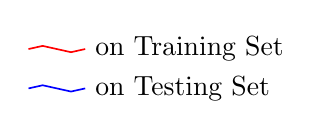
\begin{tikzpicture}
      \draw[red,semithick] (0,.5) -- (.18,.54) --
        (.54,.46) -- (.72,.5) node[right,black]
        {on Training Set};
      \draw[blue,semithick] (0,0) -- (.18,.04) --
        (.54,-.04) -- (.72,0) node[right,black]
        {on Testing Set};
    \end{tikzpicture}
  \end{flushright}
  \caption{The amount of Trees of the PCF $N$, in relation
    to $predicted$ and $accuracy$.}
  \label{fig:n}
\end{figure*}



\section{Partial Classification Forest}
\label{sec:pcf}

The PCF has two parameters, (\romannumeral 1) $N$ and
(\romannumeral 2) an array with $N$ pointers.
$N$ is the amount of Trees the PCF maintains.
Initially the pointers inside the array are references to
Nil nodes.

The PCF offers the same two operations a Tree has, FIT
(Algorithm~\ref{alg:pcf_fit}) and PREDICT (Algorithm~%
\ref{alg:pcf_pred}), both abstractions to the equivalent
Tree operations.

Once FIT is executed, the pointers are references to the
roots of fitted Tree instances.

Both FIT and PREDICT can be implemented as multi-threaded
operations as long as $\gamma$ is thread-safe, since the
Tree instances are independent of each other and the shared
parameters $X$, $y$ (FIT) and $x$ (PREDICT) are read only,
making synchronization unnecessary.

FIT first computes $\beta_X$ which has a time complexity
of:
\begin{align}
  \mathcal{O}(|\text{dimensions}(X)| * |X|).
\end{align}

After that the Tree's FIT operation is called $N$ times,
which means the PCF's FIT operation has a worst case time
complexity of:
\begin{align}
  \mathcal{O} (N * \text{FIT} + |\text{dimensions}(X)|*|X|)
\end{align}
(see Equation~\ref{eq:O_fit} for $\mathcal{O}$(FIT)).

% {{{
\begin{algorithm}
  \caption{: FIT($\Pi, X, y, \gamma, \tau_{l},
    \tau_{|X|}, \tau_{h}$)}%
  \label{alg:pcf_fit}
  The PCF's FIT operation.

  Inputs:

    \begin{tabu}{llX}
    $\Pi$ &$-$ &a PCF instance,\\
    $X$ &$-$ &input data,\\
    $y$ &$-$ &labels of X,\\
    $\gamma$ &$-$ &function returning a classifier and its
      loss,\\
    $\tau_{l}$ &$-$ &loss threshold,\\
    $\tau_{|X|}$ &$-$ &threshold for the size of X,\\
    $\tau_{h}$ &$-$ &height limit of the Tree
    \end{tabu}

  Output: void

  \noindent\rule{\linewidth}{0.4pt}

  \begin{algorithmic}[1]
    \STATE compute $\beta_X$
    \FORALL{$\Theta \in \Pi$.trees}
      \STATE{FIT($\Theta$, $X$, $y$, 0, $\beta_X$, \dots)}
    \ENDFOR
  \end{algorithmic}
\end{algorithm}
% }}}

The PCF's PREDICT operation first initializes an array with
$N$ elements (Algorithm~\ref{alg:pcf_pred}, line 1). Each
Tree instance fills one element of the array with its
prediction. After that the PCF's PREDICT operation takes
the label predicted most and returns it as its prediction
for the observation $x$ (Algorithm~\ref{alg:pcf_pred},
lines 5, 6).

The worst case time complexity of the PCF's PREDICT
operation is:
\begin{align}
  \mathcal{O}(N * (\tau_h + \mathcal{O} (\text{classifier})) + N),
\end{align}
since a Tree's PREDICT operation
is executed $N$ times, plus the most predicted label
must be determined, which is $\mathcal{O}(N)$.

% {{{
\begin{algorithm}
  \caption{: PREDICT($\Pi, x$)}
  \label{alg:pcf_pred}
  The PCF's PREDICT operation.

  Inputs:

    \begin{tabu}{llX}
    $\Pi$ &$-$ &a PCF instance,\\
    $x$ &$-$ &an observation, \\
    \end{tabu}

  Output: the predicted label or $\Lambda$

  \noindent\rule{\linewidth}{0.4pt}

  \begin{algorithmic}[1]
    \STATE predictions $\leftarrow [\Lambda; N]$
    \FOR{$i = 1$ \TO $N$}
      \STATE{predictions$[i]$ = PREDICT($\Pi$.trees$[i]$,
        $x$, $0$)}
    \ENDFOR
    \STATE determine $l_{max}$, the label predicted most
    \RETURN $l_{max}$
  \end{algorithmic}
\end{algorithm}
% }}}


\section{Tests}
\label{sec:tests}

\def\setmeshr#1{
  \def\meshr{#1}
}
\def\meshr{1pt}

\pgfooclass{meshgrid visualizer}{
  % Stores the name of the visualizer. This is needed for
  % filtering and configuration
  \attribute name;

  % The constructor. Just setup the attribute.
  \method meshgrid visualizer(#1) { \pgfooset{name}{#1} }

  % Connect to visualize signal.
  \method default connects() {
    \pgfoothis.get handle(\me)
    \pgfkeysvalueof{/pgf/data visualization/obj}.connect(
      \me,visualize,visualize datapoint signal)
  }

  % This method is invoked for each data point. It checks
  % whether the data point belongs to the correct
  % visualizer and, if so, calls the macro \dovisualization
  % to do the actual visualization.
  \method visualize() {
    \pgfdvfilterpassedtrue
    \pgfdvnamedvisualizerfilter
    \ifpgfdvfilterpassed
      \dovisualization
    \fi
  }
}

\def\dovisualization{
  \pgfkeysvalueof{%
    /data point/\pgfoovalueof{name}/execute at begin%
  }

  \pgfpointdvdatapoint
  \pgfgetlastxy{\macrox}{\macroy}

  \pgfmathsetmacro\xlow {\macrox - \meshr}
  \pgfmathsetmacro\ylow {\macroy - \meshr}
  \pgfmathsetmacro\xhigh{\macrox + \meshr}
  \pgfmathsetmacro\yhigh{\macroy + \meshr}

  \pgfpathrectanglecorners{\pgfpoint{\xlow}{\ylow}}
                          {\pgfpoint{\xhigh}{\yhigh}}

  \pgfkeysvalueof{%
    /data point/\pgfoovalueof{name}/execute at end%
  }
}
\tikzdatavisualizationset{
  visualize as meshgrid/.style={
    new object={
      when=after survey,
      store=/tikz/data visualization/visualizers/#1,
      class=meshgrid visualizer,
      arg1=#1
    },
    new visualizer={#1}{%
      color=visualizer color,
      every path/.style={fill,draw,opacity=0.5},
    }{},
    /data point/set=#1
  },
  visualize as meshgrid/.default=meshgrid
}

\setmeshr{0.5pt}

\def\visualizeds#1{
  \begin{tikzpicture}
    \datavisualization [
      scientific axes=clean,
      visualize as meshgrid/.list={mesh0, mesh1},
      visualize as scatter/.list={data0, data1},
      mesh0={style={color=red!50}},
      mesh1={style={color=blue!50}},
      data0={style={mark=o, mark size=0.1pt,
        visualizer color=red}},
      data1={style={mark=o, mark size=0.1pt,
        visualizer color=blue}},
    ]
    data[headline={x, y}, read from file=#1.mesh_0.csv,
      set=mesh0]
    data[headline={x, y}, read from file=#1.mesh_1.csv,
      set=mesh1]
    data[headline={x, y}, read from file=#1.data_0.csv,
      set=data0]
    data[headline={x, y}, read from file=#1.data_1.csv,
      set=data1]
    ;
  \end{tikzpicture}
}

\begin{figure*}

  \begin{comment}
  \begin{subfigure}[b]{0.3\textwidth}
    \centering
    \scalebox{0.75}{\visualizeds{tests/data/e2_ls2}}
    \caption{$\tau_{|X|} = 2$, $N = 2$}
  \end{subfigure}
  \begin{subfigure}[b]{0.3\textwidth}
    \centering
    \scalebox{0.75}{\visualizeds{tests/data/e5_ls2}}
    \caption{$\tau_{|X|} = 2$, $N = 5$}
  \end{subfigure}
  \begin{subfigure}[b]{0.3\textwidth}
    \centering
    \scalebox{0.75}{\visualizeds{tests/data/e10_ls2}}
    \caption{$\tau_{|X|} = 2$, $N = 10$}
  \end{subfigure}

  \begin{subfigure}[b]{0.3\textwidth}
    \centering
    \scalebox{0.75}{\visualizeds{tests/data/e2_ls5}}
    \caption{$\tau_{|X|} = 5$, $N = 2$}
  \end{subfigure}
  \begin{subfigure}[b]{0.3\textwidth}
    \centering
    \scalebox{0.75}{\visualizeds{tests/data/e5_ls5}}
    \caption{$\tau_{|X|} = 5$, $N = 5$}
  \end{subfigure}
  \begin{subfigure}[b]{0.3\textwidth}
    \centering
    \scalebox{0.75}{\visualizeds{tests/data/e10_ls5}}
    \caption{$\tau_{|X|} = 5$, $N = 10$}
  \end{subfigure}

  \begin{subfigure}[b]{0.3\textwidth}
    \centering
    \scalebox{0.75}{\visualizeds{tests/data/e2_ls10}}
    \caption{$\tau_{|X|} = 10$, $N = 2$}
  \end{subfigure}
  \begin{subfigure}[b]{0.3\textwidth}
    \centering
    \scalebox{0.75}{\visualizeds{tests/data/e5_ls10}}
    \caption{$\tau_{|X|} = 10$, $N = 5$}
  \end{subfigure}
  \begin{subfigure}[b]{0.3\textwidth}
    \centering
    \scalebox{0.75}{\visualizeds{tests/data/e10_ls10}}
    \caption{$\tau_{|X|} = 10$, $N = 10$}
  \end{subfigure}
  \end{comment}

  \begin{flushright}
  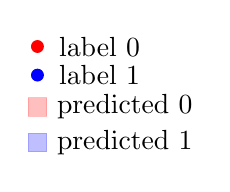
\begin{tikzpicture}
    \begin{scope}[label distance=2pt]
    \node[color=red, circle, draw,fill,label=right:label 0,
      inner sep=1.5pt] at (0,0) (l_zero) {};
    \node[color=blue, circle,draw,fill,label=right:label 1,
      below=0.2 of l_zero, inner sep=1.5pt] (l_one) {};
    \end{scope}
    \node[color=red!50,opacity=0.5,label=right:predicted 0,
      below=0.2 of l_one, fill, draw] (m_zero) {};
    \node[color=blue!50,opacity=0.5,below=0.2 of m_zero,
      label=right:predicted 1, fill, draw] (m_one) {};
  \end{tikzpicture}
  \end{flushright}

\end{figure*}

\section{Further optimizations and additional features}
\label{sec:oandf}

\section{Conclusion}
\label{sec:conclusion}

\bibliography{pcf}

\end{document}
